\documentclass{assignment}
\UsingEnglish
\ProjectInfos*{Intro to Communication System}{EE140}{Fall, 2020}{Assignment 9}{Due time : 10:15, Dec 4, 2020 (Friday)}{陈稼霖}{45875852}
\begin{document}
\begin{prob}[3.1]
    Let $U$ be an analog rv uniformly distributed between $-1$ and $1$.
    \begin{itemize}
        \item[(a)] Find the $3$-bit ($M=8$) quantizer that minimizes the MSE.
        \item[(b)] Argue that your quantizer satisfies the necessary condition for optimality.
        \item[(c)] Show that the quantizer is unique in the sense that no other $3$-bit quantizer satisfies the necessary condition for optimality.
    \end{itemize}
\end{prob}
\begin{sol}
    \begin{itemize}
        \item[(a)] The $3$-bit quantizer that minimizes the MSE for the uniformly distributed analog rv $U$ should be a uniform quantizer with $8$ equally-spaced quantization intervals bounded by endpoints
        \begin{align}
            \label{P-1-endpoints}
            b_0=-1,\quad b_1=-\frac{3}{4},\quad b_2=-\frac{1}{2},\quad b_3=-\frac{1}{4},\quad b_4=0,\quad b_5=\frac{1}{4},\quad b_6=\frac{1}{2},\quad b_7=\frac{3}{4},\quad b_8=1
        \end{align}
        and $8$ equally-spaced representation points
        \begin{align}
            \label{P-1-representation-points}
            a_1=-\frac{7}{8},\quad a_2=-\frac{5}{8},\quad a_3=-\frac{3}{8},\quad a_4=-\frac{1}{8},\quad a_5=\frac{1}{8},\quad a_6=\frac{3}{8},\quad a_7=\frac{5}{8},\quad a_8=\frac{7}{8}.
        \end{align}
        \item[(b)] The above uniform quantizer satisfies the Lloyd-Max necessary conditions:
        \begin{itemize}
            \item[(i)] For the given representation points $\{a_j\}$, the interval endpoints (excepts the first and the last ones) are the midpoints of the neighboring representation points:
            \begin{align}
                \label{P-1-necessary-condition-1}
                b_j=\frac{a_j+a_{j+1}}{2},\quad\forall j=1,2,\cdots,7.
            \end{align}
            \item[(ii)] For the given quantization intervals $\{(b_j,b_{j+1})\}$, the representation points are the expectation of the analog rv in the corresponding quantization intervals
            \begin{align}
                \label{P-1-necessary-condition-2}
                \notag a_j=E[U\vert U\in\mathcal{R}_j]=\frac{\int_{\mathcal{R}_j}f_U(u)u\,\mathrm{d}u}{\int_{\mathcal{R}_j}}f_U(u)\,\mathrm{d}u=\frac{\int_{u_{j-1}}^{u_j}\frac{1}{2}u\,\mathrm{d}u}{\int_{u_{j-1}}^{u_j}\frac{1}{2}\,\mathrm{d}u}=\frac{\frac{1}{2}(b_j^2-b_{j-1}^2)}{\frac{1}{2}(b_j-b_{j-1})}=\frac{1}{2}(b_j+b_{j+1}),\\
                \forall j=1,2\cdots,8.
            \end{align}
        \end{itemize}
        \item[(c)] Plugging equation \eqref{P-1-necessary-condition-2} into equation \eqref{P-1-necessary-condition-1}, we get
        \begin{align}
            b_j=\frac{\frac{b_{j-1}+b_j}{2}+\frac{b_j+b_{j+1}}{2}}{2}=\frac{1}{4}b_{j-1}+\frac{1}{2}b_j+\frac{1}{4}b_{j+1}\Longrightarrow b_{j+1}-b_j=b_j-b_{j-1},\quad\forall j=1,2,\cdots,7,
        \end{align}
        which means that for any $3$-bit quantizers satisfying the necessary condition, it must have equally-spaced quantization intervals bounded by endpoints as equation \eqref{P-1-endpoints} shows. Besides, according to equation \eqref{P-1-necessary-condition-2}, for any $3$-bit quantizers satisfying the necessary condition, it must have equally-spaced representation points as equation \eqref{P-1-representation-points} shows.\\
        Therefore, there is only one $3$-bit quantizer that minimize the MSE --- the one with $8$ equally-spaced quantization intervals and $8$ equally-spaced representation points. It is unique.
    \end{itemize}
\end{sol}

\begin{prob}[3.3]
    Consider a binary scalar quantizer that partitions the set of reals $\mathbb{R}$ into two subsets $(-\infty,b]$ and $(b,\infty)$ and then presents $(-\infty,b]$ by $a_1\in\mathbb{R}$ and $(b,\infty)$ by $a_2\in\mathbb{R}$. This quantizer is used on each letter $U_n$ of a sequence $\cdots,U_{-1},U_0,U_1,\cdots$ of iid random variables, each having the probability density $f(u)$. Assume throughout this exercise that $f(u)$ is symmetric, i.e. that $f(u)=f(-u)$ for all $u\geq 0$.
    \begin{itemize}
        \item[(a)] Given the representation levels $a_1$ and $a_2>a_1$, how should $b$ be chosen to minimize the mean-squared distortion in the quantization? Assume that $f(u)>0$ for $a_1\leq u\leq a_2$ and explain why this assumption is relevant.
        \item[(b)] Given $b\geq 0$, find the values of $a_1$ and $a_2$ that minimize the mean-squared distortion. Given both answer in terms of the two functions $Q(x)=\int_x^{\infty}f(u)\,\mathrm{d}u$ and $y(x)=\int_x^{\infty}uf(u)\,\mathrm{d}u$.
        \item[(c)] Show that for $b=0$, the minimizing values of $a_1$ and $a_2$ satisfy $a_1=-a_2$.
        \item[(d)] Show that the choice of $b$, $a_1$, and $a_2$ in part (c) satisfies the Lloyd-Max conditions for minimum mean-squared distortion.
        \item[(e)] Consider the particular symmetric density
        \begin{figure}[H]
            \centering
            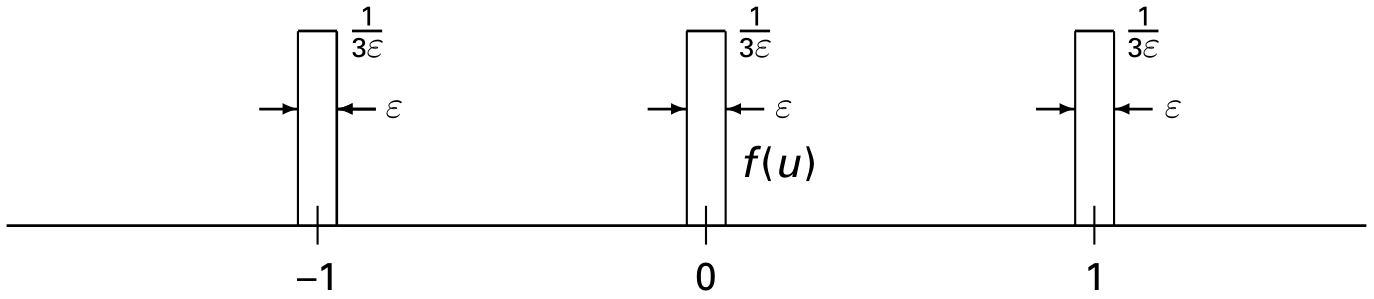
\includegraphics[width=.5\columnwidth]{A-9-P-1.png}
            \caption{}
            \label{A-9-P-1}
        \end{figure}
        Find all sets of triples $\{b,a_1,a_2\}$ that satisfy the Lloyd-Max conditions and evaluate the MSE for each. You are welcome in your calculation to replace each region of nonzero probability density above with an impulse, i.e. $f(u)=(1/3)[\delta(-1)+\delta(0)+\delta(1)]$, but you should use Figure \ref{A-9-P-1} to resolve the ambiguity about regions that occurs when $b$ is $-1,0$ or $+1$.
        \item[(f)] Given the MSE for each of your solutions above (in the limit of $\varepsilon\rightarrow 0$). Which of your solutions minimizes the MSE?
    \end{itemize}
\end{prob}
\begin{sol}
    \begin{itemize}
        \item[(a)] The mean-squared distortion is
        \begin{align}
            \text{MSE}=E[\abs{U-V}^2]=\int_{-\infty}^bf(u)(u-a_1)^2\,\mathrm{d}u+\int_b^{+\infty}f(u)(u-a_2)^2\,\mathrm{d}u.
        \end{align}
        Given $a_1$ and $a_2$, to minimize the mean-squared distortion, we require that
        \begin{align}
            \label{P-2-necessary-condition}
            \frac{\partial\text{MSE}}{\partial b}=f(b)(b-a_1)^2-f(b)(b-a_2)^2=2(a_1-a_2)f(b)\left(\frac{a_1+a_2}{2}-b\right)=0.
        \end{align}
        Here, $a_1-a_2\neq 0$. Under the assumption that $f(u)>0$, we need that
        \begin{align}
            b=\frac{a_1+a_2}{2},
        \end{align}
        which means that we quantize $u$ to the nearest representation point.

        The above assumption is relevant, since if $\exists u_0\in[a_1,a_2]$ such that $f(u_0)=0$, then $b=u_0$ is also a solution to equation \eqref{P-2-necessary-condition}. However, this solution, $b=u_0$, may not necessarily guarantee that we can quantize $u$ to the nearest representation point and thus can not minimize the mean-squared distortion. Besides, consider such a case that $f(u)=0\forall a_1\leq u\leq a_2$. In this case, we can choose any $b\in[a_1,a_2]$ to minimize the mean-squared distortion, not necessarily $b=\frac{a_1+a_2}{2}$.
        \item[(b)] Given $b$, to minimize the mean-squared distortion, we require that
        \begin{gather}
            \frac{\partial\text{MSE}}{\partial a_1}=-2\int_{-\infty}^bf(u)(u-a_1)\,\mathrm{d}u=0,\\
            \Longrightarrow a_1=\frac{\int_{-\infty}^bf(u)u\,\mathrm{d}u}{\int_{-\infty}^bf(u)\,\mathrm{d}u}=\frac{-\int_{-b}^{+\infty}f(u)u\,\mathrm{d}u}{1-\int_b^{\infty}f(u)\,\mathrm{d}u}=-\frac{y(-b)}{1-Q(b)}=-\frac{y(b)}{1-Q(b)}.
        \end{gather}
        and that
        \begin{gather}
            \frac{\partial\text{MSE}}{\partial a_2}=-2\int_b^{+\infty}f(u)(u-a_2)\,\mathrm{d}u=0,\\
            \Longrightarrow a_2=\frac{\int_b^{+\infty}f(u)u\,\mathrm{d}u}{\int_b^{+\infty}f(u)\,\mathrm{d}u}=\frac{y(b)}{Q(b)}.
        \end{gather}
        \item[(c)] Since $f(u)=f(-u)\forall u\geq 0$, we have
        \begin{align}
            \notag Q(0)=&\int_0^{+\infty}f(u)\,\mathrm{d}u=\frac{1}{2}\int_0^{+\infty}f(u)\,\mathrm{d}u+\frac{1}{2}\int_0^{+\infty}f(u)\,\mathrm{d}u=\frac{1}{2}\int_0^{+\infty}f(u)\,\mathrm{d}u+\frac{1}{2}\int_{-\infty}^0f(u)\,\mathrm{d}u\\
            =&\frac{1}{2}\int_{-\infty}^{+\infty}f(u)\,\mathrm{d}u=\frac{1}{2}.
        \end{align}
        For $b=0$,
        \begin{align}
            a_1=-\frac{y(0)}{1-Q(0)}=-2y(0),
        \end{align}
        and
        \begin{align}
            a_2=\frac{y(0)}{Q(0)}=2y(0),
        \end{align}
        so
        \begin{align}
            a_1=-a_2.
        \end{align}
        \item[(d)] The choice of $b$, $a_1$, and $a_2$ in part (c) satisfies the Lloyd-Max conditions for minimum mean-squared distortion:
        \begin{itemize}
            \item[(i)] The quantization interval endpoint $b$ is the midpoint of the representation points $a_1$ and $a_2$:
            \begin{align}
                b=0=\frac{a_1+a_2}{2}.
            \end{align}
            \item[(ii)] The representation points $a_1$ and $a_2$ are the expectation of the random variable $U$ in their corresponding quantization intervals:
            \begin{align}
                a_1=\frac{\int_{-\infty}^0f(u)u\,\mathrm{d}u}{\int_{-\infty}^0f(u)\,\mathrm{d}u}=E[U\vert U\leq 0].
            \end{align}
            and
            \begin{align}
                a_2=\frac{\int_0^{+\infty}f(u)u\,\mathrm{d}u}{\int_0^{+\infty}f(u)\,\mathrm{d}u}=E[U\vert U>0].
            \end{align}
        \end{itemize}
        \item[(e)] For this particular symmetric density,
        \begin{align}
            y(x)=\left\{\begin{array}{ll}
                0,&x\leq-1-\varepsilon/2,\\
                \frac{1}{3}+\frac{1}{6\varepsilon}[(-1+\varepsilon/2)^2-x^2],&-1-\varepsilon/2<x\leq-1+\varepsilon/2,\\
                \frac{1}{3},&-1+\varepsilon/2<x\leq-\varepsilon/2,\\
                \frac{1}{3}+\frac{1}{6\varepsilon}[(\varepsilon/2)^2-x^2],&-\varepsilon/2<x\leq\varepsilon/2,\\
                \frac{1}{3},&\varepsilon/2<x\leq 1-\varepsilon/2,\\
                \frac{1}{6\varepsilon}[(1+\varepsilon/2)^2-x^2],&1-\varepsilon/2<x\leq 1+\varepsilon/2,\\
                0,&x>1+\varepsilon/2,
            \end{array}\right.
        \end{align}
        and
        \begin{align}
            Q(x)=\left\{\begin{array}{ll}
                1,&x\leq-1-\varepsilon/2,\\
                1-\frac{1}{3\varepsilon}[x-(-1-\varepsilon/2)],&-1-\varepsilon/2<x\leq-1+\varepsilon/2,\\
                \frac{2}{3},&-1+\varepsilon/2<x\leq-\varepsilon/2,\\
                \frac{2}{3}-\frac{1}{3\varepsilon}[x-(-\varepsilon/2)],&-\varepsilon/2<x\leq\varepsilon/2,\\
                \frac{1}{3},&\varepsilon/2<x\leq 1-\varepsilon/2,\\
                \frac{1}{3}-\frac{1}{3\varepsilon}[x-(1-\varepsilon/2)],&1-\varepsilon/2<x\leq 1+\varepsilon/2,\\
                0,&x>1+\varepsilon/2.
            \end{array}\right.,
        \end{align}
        so
        \begin{align}
            -\frac{y(x)}{1-Q(x)}=\left\{\begin{array}{ll}
                \frac{1}{2}[x-(1+\varepsilon/2)],&-1-\varepsilon/2<x\leq-1+\varepsilon/2,\\
                -1,&-1+\varepsilon/2<x\leq-\varepsilon/2,\\
                \frac{x^2-(\varepsilon/2)^2-2\varepsilon}{2x+3\varepsilon},&-\varepsilon/2<x\leq\varepsilon/2,\\
                -\frac{1}{2},&\varepsilon/2<x\leq 1-\varepsilon/2,\\
                \frac{x^2-(1+\varepsilon/2)^2}{2x+5\varepsilon-2},&1-\varepsilon/2<x1+\varepsilon/2,\\
                0,&x>1+\varepsilon/2,
            \end{array}\right.
        \end{align}
        and
        \begin{align}
            \frac{y(x)}{Q(x)}=\left\{\begin{array}{ll}
                0,&x\leq 1-\varepsilon/2,\\
                \frac{-x^2+(1+\varepsilon/2)^2}{-2x+3\varepsilon},&-1-\varepsilon/2<x\leq-1+\varepsilon/2,\\
                \frac{1}{2},&-1+\varepsilon/2<x\leq-\varepsilon/2,\\
                \frac{x^2-(\varepsilon/2)^2-2\varepsilon}{2x-3\varepsilon},&-\varepsilon/2<x\leq\varepsilon/2,\\
                1,&\varepsilon/2<x\leq 1-\varepsilon/2,\\
                \frac{x^2-(1+\varepsilon/2)^2}{2x-\varepsilon-2},&1-\varepsilon/2<x\leq 1+\varepsilon/2.
            \end{array}\right.
        \end{align}
        Sets of triple $\{b,a_1,a_2\}$ satisfying the Lloyd-Max conditions are (assuming $\epsilon\rightarrow 0$):
        \begin{itemize}
            \item[(i)] $b=0,a_1=-\frac{2}{3},a_2=\frac{2}{3}$;
            \item[(ii)] $b=-\frac{1}{4},a_1=-1,a_2=\frac{1}{2}$;
            \item[(iii)] $b=\frac{1}{4},a_1=-\frac{1}{2},a_2=1$.
        \end{itemize}
        \item[(f)] 
        \begin{itemize}
            \item[(i)] For $b=0,a_1=-\frac{2}{3},a_2=\frac{2}{3}$,
            \begin{align}
                \text{MSE}=\lim_{b\rightarrow 0}\int_{-\infty}^0f(u)(u+\frac{2}{3})^2\,\mathrm{d}u+\int_0^{+\infty}f(u)(u-\frac{2}{3})^2\,\mathrm{d}u=\frac{2}{9}.
            \end{align}
            \item[(ii)] For $b=-\frac{1}{4},a_1=-1,a_2=\frac{1}{2}$,
            \begin{align}
                \text{MSE}=\lim_{b\rightarrow 0}\int_{-\infty}^{-\frac{1}{4}}f(u)(u+1)^2\,\mathrm{d}u+\int_{-\frac{1}{4}}^{+\infty}f(u)(u-\frac{1}{2})^2\,\mathrm{d}u=\frac{1}{6}.
            \end{align}
            \item[(iii)] For $b=\frac{1}{4},a_1=-\frac{1}{2},a_2=1$,
            \begin{align}
                \text{MSE}=\lim_{b\rightarrow 0}\int_{-\infty}^{\frac{1}{4}}f(u)(u+\frac{1}{2})^2\,\mathrm{d}u+\int_{\frac{1}{4}}^{+\infty}f(u)(u-1)^2\,\mathrm{d}u=\frac{1}{6}.
            \end{align}
        \end{itemize}
        The solutions (ii) ($b=-\frac{1}{4},a_1=-1,a_2=\frac{1}{2}$) and (iii) ($b=\frac{1}{4},a_1=-\frac{1}{2},a_2=1$) minimize the MSE.
    \end{itemize}
\end{sol}

\begin{prob}[3.4]
    Section 3.4 partly analyzed a minimum-MSE quantizer for a pdf in which $f_U(u)=f_1$ over an interval of size $L_1$, $f_U(u)=f_2$ over an interval of size $L_2$, and $f_U(u)=0$ elsewhere. Let $M$ be the total number of representation points to be used, with $M_1$ in the first interval and $M_2=M-M_1$ in the second. Assume (from symmetry) that the quantization intervals are of equal size $\Delta_1=L_1/M_1$ in interval $1$ and of equal size $\Delta_2=L_2/M_2$ in interval $2$. Assume that $M$ is very large, so that we can approximately minimize the MSE over $M_1$, $M_2$ without an integer constraint on $M_1$, $M_2$ (that is, assume that $M_1$, $M_2$ can be arbitrary real numbers).
    \begin{itemize}
        \item[(a)] Show that the MSE is minimized if $\Delta_1f_1^{1/3}=\Delta_2f_2^{1/3}$, i.e. the quantization interval sizes are inversely proportional to the cube root of the density. [Hint. Use a Lagrange multiplier to perform the minimization. That is, to minimize a function MSE$(\Delta_1,\Delta_2)$ subject to a constraint $M=f(\Delta_1,\Delta_2)$, first minimize MSE$(\Delta_1,\Delta_2)+\lambda f(\Delta_1,\Delta_2)$ without the constraint, and, second, choose $\lambda$ so that the solution meets the constraint.]
        \item[(b)] Show that the minimum MSE under the above assumption is given by
        \[
            \text{MSE}=\frac{(L_1f_1^{1/3}+L_2f_2^{1/3})^3}{12M^2}.
        \]
        \item[(c)] Assume that the Lloyd-Max algorithm is started with $0<M_1<M$ representation points in the first interval and $M_2=M-M_1$ points in the second interval. Explain where the Lloyd-Max algorithm converges for this starting point. Assume from here on that the distance between the two intervals is very large.
        \item[(d)] Redo part (c) under the assumption that the Lloyd-Max algorithm is started with $0<M_1<M-2$ representation points in the first interval, one point between the two intervals, and the remaining points in the second interval.
        \item[(e)] Express the exact minimum MSE as a minimum over $M-1$ possibilities, with one term for each choice of $0<M_1<M$. (Assume there are no representation points between the two intervals.)
        \item[(f)] Now consider an arbitrary choice of $\Delta_1$ and $\Delta_2$ (with no constraint on $M$). Show that the entropy of the set of quantization points is given by
        \[
            H(V)=-f_1L_1\log(f_1\Delta_1)-f_2L_2\log(f_2\Delta_2).
        \]
        \item[(g)] Show that if the MSE is minimized subject to a constraint on the entropy (ignoring the integer constraint on quantization level), then $\Delta_1=\Delta_2$.
    \end{itemize}
\end{prob}
\begin{sol}
    \begin{itemize}
        \item[(a)] The MSE of the quantization is
        \begin{align}
            \label{P-3-MSE}
            \notag\text{MSE}=&E[(U-V)^2]=\sum_{i=1,2}\sum_{j=1}^{M_i}\int_{a_j^{(i)}-\frac{1}{2}\Delta_i}^{a_j^{(i)}+\frac{1}{2}\Delta_i}f_i\left[u-a_j^{(i)}\right]^2\,\mathrm{d}u\\
            \notag=&\sum_{j=1}^{M_1}\int_{a_j-\frac{1}{2}\Delta_1}^{a_j+\frac{1}{2}\Delta_1}f_1\left[u-a_j^{(1)}\right]^2\,\mathrm{d}u+\sum_{j=1}^{M_2}\int_{a_j^{(2)}-\frac{1}{2}\Delta_2}^{a_j^{(2)}+\frac{1}{2}\Delta_2}f_2\left[u-a_j^{(2)}\right]^2\,\mathrm{d}u\\
            \notag=&M_1f_1\frac{\Delta_1^3}{12}+M_2f_2\frac{\Delta_2^3}{12}\\
            =&f_1L_1\frac{\Delta_1^2}{12}+f_2L_2\frac{\Delta_2^2}{12},
        \end{align}
        where $a_j^{(i)}$ is the $j$th representation point in the $i$th interval.
        The constraint is
        \begin{align}
            \label{P-3-constraint}
            M=f(\Delta_1,\Delta_2)=\frac{L_1}{\Delta_1}+\frac{L_2}{\Delta_2}.
        \end{align}
        To minimize $\text{MSE}+\lambda f(\Delta_1,\Delta_2)$, we have
        \begin{align}
            \frac{\partial}{\partial\Delta_1}[\text{MSE}+\lambda f(\Delta_1,\Delta_2)]=&\frac{1}{6}f_1L_1\Delta_1-\frac{\lambda L_1}{\Delta_1^2}=0,\\
            \frac{\partial}{\partial\Delta_2}[\text{MSE}+\lambda f(\Delta_1,\Delta_2)]=&\frac{1}{6}f_1L_1\Delta_1-\frac{\lambda L_2}{\Delta_2^2}=0.
        \end{align}
        \begin{gather}
            \label{P-3-Lagrange-result}\Longrightarrow\lambda=\frac{1}{6}f_1\Delta_1^3=\frac{1}{6}f_1\Delta_2^3,\\
            \Longrightarrow\Delta_1f_1^{1/3}=\Delta_2f_2^{1/3}.
        \end{gather}
        Therefore, MSE is minimized if $\Delta_1f_1^{1/3}=\Delta_2f_2^{1/3}$.
        \item[(b)] From equation \ref{P-3-Lagrange-result} together with the constraint \ref{P-3-constraint}, we get
        \begin{align}
            \lambda=&\frac{(L_1f_1^{1/3}+L_2f_2^{1/3})^3}{6M^3},\\
            \Delta_1=&\frac{L_1f_1^{1/3}+L_2f_2^{1/3}}{Mf_1^{1/3}},\\
            \Delta_2=&\frac{L_1f_2^{1/3}+L_2f_2^{1/3}}{Mf_2^{1/3}}.
        \end{align}
        so the minimized MSE under the above assumption is
        \begin{align}
            \text{MSE}=\frac{f_1L_1^{1/3}(L_1f_1^{1/3}+L_2f_2^{1/3})^2}{M^2}+\frac{f_2L_2^{1/3}(L_1f_1^{1/3}+L_2f_2^{1/3})^2}{M^2}=\frac{(L_1f_1^{1/3}+f_2f_2^{1/3})^3}{M^2}.
        \end{align}
        \item[(c)] The Lloyd-Max algorithm converges at such a scheme:
        \begin{align*}
            \text{representation points}:&\overbrace{u_1+\frac{L_1}{2M_1},\quad u_1+3\frac{L_1}{2M_1},\quad\cdots,\quad u_1+(2M_1-3)\frac{L_1}{2M_1},\quad u_1+(2M_1-1)\frac{L_2}{2M_1}}^{M_1 \text{ uniformly-spaced representation points in the first interval}},\\
            &\overbrace{u_2+\frac{L_2}{2M_2},\quad u_2+3\frac{L_2}{2M_2},\quad\cdots,\quad u_2+(2M_2-3)\frac{L_2}{2M_2},\quad u_2+(2M_2-1)\frac{L_2}{2M_2}}^{M_2 \text{ uniformly-spaced representation points in the second interval}},\\
            \text{quantization intervals}:&
        \end{align*}
        {\scriptsize
        \begin{align*}
            &\overbrace{\left[u_1,u_1+\frac{L_1}{M_1}\right],\left(u_1+\frac{L_1}{M},u_1+2\frac{L_1}{M_1}\right],\cdots,\left(u_1+(M_1-2)\frac{L_1}{M_1},u_1+(M_1-1)\frac{L_1}{M_1}\right]}^{M_1-1\text{ uniformly distributed quantization intervals in the first interval}},\overbrace{\left(u_1+(M_1-1)\frac{L_1}{M_1},\frac{u_1+(M_1-\frac{1}{2})\frac{L_1}{M_1}+u_2+\frac{1}{2}\frac{L_2}{M_2}}{2}\right]}^{M_1\text{th quantization interval}}\\
            &\overbrace{\left(\frac{u_1+(M_1-\frac{1}{2})\frac{L_1}{M_1}+u_2+\frac{1}{2}\frac{L_2}{M_2}}{2},u_2+\frac{L_2}{M_2}\right]}^{M_1+1\text{th quantization interval}},\overbrace{\left(u_2+\frac{L_2}{M_2},u_2+2\frac{L_2}{M_2}\right],\cdots,\left(u_2+(M_2-2)\frac{L_2}{M_2},u_2+(M_2-1)\frac{L_2}{M_2}\right],\left(u_2+(M_2-1)\frac{L_2}{M_2},u_2+L_2\right]}^{M_2-1\text{ uniformly distributed quantization intervals in the second interval}}.
        \end{align*}
        }%
        where $[u_1,u_1+L_1]$ is the first interval and $[u_2+L_2]$ is the second interval.\\
        Explanation: if the Lloyd-Max algorithm starts with $0<M_1<M$ representation points in the first interval and $M_2=M-M_1$ points in the second interval, the second step of Lloyd-Max algorithm (choose the boundary points of the quantization intervals as the midpoints of the neighboring representation points) will remain the first $M_1$ boundary points of the quantization intervals in the first interval, last $M_2$ boundary points of quantization intervals in the second interval and the $M_1+1$th boundary point of the interval in the gap between the two intervals. The third step (choose the representation points as the expectation of $U$ in their corresponding quantization intervals) will remain the first $M_1$ representation points in the first interval and the last $M_2$ representation points in the second interval. Repeating the Lloyd-Max algorithm, eventually, we will reach the quantizer scheme described above, since it satisfies the Lloyd-Max conditions.
        \item[(d)] The Lloyd-Max algorithm will end in such a scheme:
        {\scriptsize
        \begin{align*}
            &\text{representation points}:\overbrace{u_1+\frac{L_1}{2M_1},\quad u_1+3\frac{L_1}{2M_1},\quad\cdots,\quad u_1+(2M_1-3)\frac{L_1}{2M_1},\quad u_1+(2M_1-1)\frac{L_1}{2M_1}}^{M_1\text{ uniformly-spaced representation points in the first interval}},\overbrace{u_0}^{\text{initial position of the }M_1+1\text{th representation points}},\\
            &\overbrace{u_2+\frac{L_2}{2(M-M_1-1)},\quad u_2+3\frac{L_2}{2(M-M_1-1)},\quad\cdots,\quad u_2+[2(M-M_1)-5]\frac{L_2}{2(M-M_1-1)},\quad u_2+[2(M-M_1)-3]\frac{L_2}{2(M-M_1-1)}}^{M-M_1-1\text{ uniformly-spaced representation points in the second interval}},\\
            &\text{quantization intervals}:
        \end{align*}
        \begin{align*}
            &\overbrace{\left[u_1,u_1+\frac{L_1}{M_1}\right],\left(u_1+\frac{L_1}{M},u_1+2\frac{L_1}{M_1}\right],\cdots,\left(u_1+(M_1-2)\frac{L_1}{M_1},u_1+(M_1-1)\frac{L_1}{M_1}\right]}^{M_1-1\text{ uniformly distributed quantization intervals in the first interval}},\overbrace{\left(u_1+(M_1-1)\frac{L_1}{M_1},\frac{u_1+(M_1-\frac{1}{2})\frac{L_1}{M_1}+u_0}{2}\right]}^{M_1\text{th quantization interval}},\\
            &\overbrace{\left(\frac{u_1+(M_1-\frac{1}{2})\frac{L_1}{M_1}+u_0}{2},\frac{u_0+u_2+\frac{L_2}{2(M-M_1-1)}}{2}\right]}^{(M_1+1)\text{th quantization interval}},\overbrace{\left(\frac{u_0+u_2+\frac{L_2}{2(M-M_1-1)}}{2},u_2+\frac{L_2}{M-M_1-1}\right]}^{(M_1+2)\text{th quantization interval}},\\
            &\overbrace{\left(u_2+\frac{L_2}{M-M_1-1},u_2+2\frac{L_2}{M-M_1-1}\right],\left(u_2+2\frac{L_2}{M-M_1-1},u_2+3\frac{L_2}{M-M_1-1}\right],\cdots,\left(u_2+(M-M_1-2)\frac{L_2}{M-M_1-1},u_2+L_2\right]}^{M-M_1-1\text{ uniformly distributed quantization quantization intervals in the second interval}}.
        \end{align*}
        }%
        where the coordinate of the $M_1+1$th representation $u_0$ remains its initial value, since the Lloyd algorithm is not well-defined within the interval where the pdf is $0$. Other representation points and quantization intervals converges similarly as (c).
        \item[(e)] Now $M_1$ and $M_2$ are integers, so equation \ref{P-3-MSE} can be expressed as
        \begin{align}
            \text{MSE}=\frac{f_1L_1^3}{12M_1^2}+\frac{f_2L_2^3}{12M_2^2}.
        \end{align}
        \item[(f)] The entropy of the set of quantization points is
        \begin{align}
            H(V)=-\sum_{i=1,2}M_if_i\Delta_i\log_2(f_i\Delta_i)=-f_1L_1\log_2(f_1\Delta_1)-f_2L_2\log_2(f_2\Delta_2).
        \end{align}
        \item[(g)] To minimize MSE under a constraint on the entropy, we have
        \begin{align}
            \frac{\partial}{\partial\Delta_1}[\text{MSE}+\lambda H(V)]=&\frac{1}{6}f_1L_1\Delta_1-\frac{\lambda f_1L_1}{\Delta_1}=0,\\
            \frac{\partial}{\partial\Delta_2}[\text{MSE}+\lambda H(V)]=&\frac{1}{6}f_2L_2\Delta_2-\frac{\lambda f_2L_2}{\Delta_2}=0,
        \end{align}
        \begin{align}
            \Longrightarrow\Delta_1=\Delta_2=\sqrt{6\lambda}.
        \end{align}
    \end{itemize}
\end{sol}

\begin{prob}[3.5]
    \begin{itemize}
        \item[(a)] Assume that a continuous-valued rv $Z$ has probability density that is $0$ except over the interval $[-A,+A]$. Show that the differential entropy $h(Z)$ is upperbounded $1+\log_2A$.
        \item[(b)] Show that $h(Z)=1+\log_2A$ if and only if $Z$ is uniformly distributed between $-A$ and $+A$.
    \end{itemize}
\end{prob}
\begin{sol}
    \begin{itemize}
        \item[(a)] 
        \item[(b)] 
    \end{itemize}
\end{sol}
\end{document}